\documentclass[12pt,letterpaper]{exam}
\usepackage[lmargin=1in,rmargin=1in,tmargin=1in,bmargin=1in]{geometry}
\usepackage{../style/exams}

% -------------------
% Course & Exam Information
% -------------------
\newcommand{\course}{MATH 111I: Exam 3}
\newcommand{\term}{Spring --- 2025}
\newcommand{\examdate}{04/17/2025}
\newcommand{\timelimit}{75 Minutes}

\setbool{hideans}{false} % Student: True; Instructor: False

% -------------------
% Content
% -------------------
\begin{document}

\examtitle
\instructions{Write your name on the appropriate line on the exam cover sheet. This exam contains \numpages\ pages (including this cover page) and \numquestions\ questions. Check that you have every page of the exam. Answer the questions in the spaces provided on the question sheets. Be sure to answer every part of each question and show all your work. If you run out of room for an answer, continue on the back of the page --- being sure to indicate the problem number.} 
\scores
\bottomline
\newpage


% -------------------
% Questions
% -------------------
\begin{questions}

% Question 1
\newpage
\question[10] Consider the exponential function $y= 3(2^{1-x})$.
	\begin{enumerate}[(a)]
	\item Write this exponential function in the form $y= Ab^x$. \pspace
	\sol{Observe that we have\dots
		\[
		y= 3(2^{1 - x})= 3(2^1 \cdot 2^{-x})= (3 \cdot 2) \cdot 2^{-x}= 6 (2^{-x})= 6(2^{-1})^x= 6 \left( \dfrac{1}{2} \right)^x
		\]
	Therefore, this function is exponential with $A= 6$ and $b= \dfrac{1}{2}$.
	} \vfill
	
	\item What is the $y$-intercept of this function? \pspace
	\sol{We know that the $y$-intercept for an exponential function of the form $y= Ab^x$ is $A$. We know from (a) that $A= 6$. Therefore, the $y$-intercept is $y= 6$, i.e. the point $(0, 6)$. Alternatively, the $y$-intercept is the value when $x= 0$. But then\dots
		\[
		y(0)= 3(2^{1-0})= 3(2^1)= 3(2)= 6
		\]
	} \vfill
	
	\item Sketch this function below. 
		\[
            	\fbox{
            	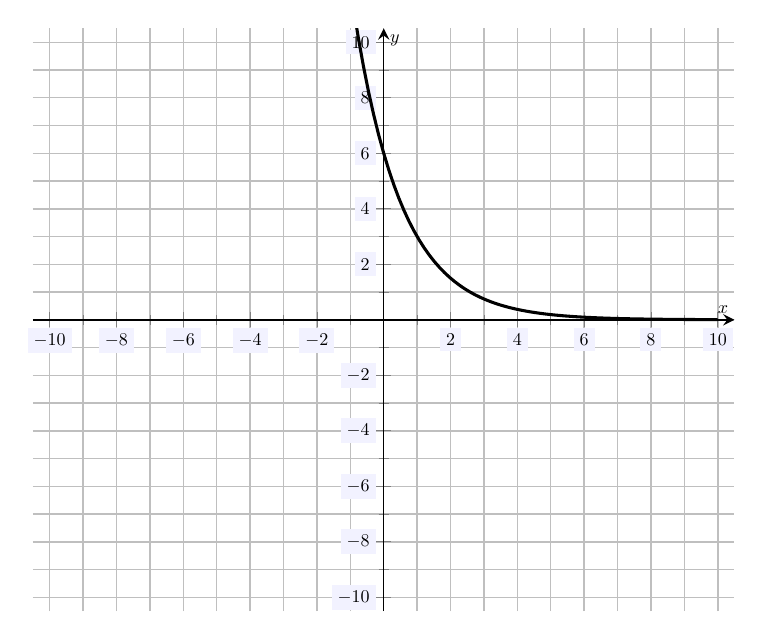
\begin{tikzpicture}[scale=1.3,every node/.style={scale=0.5}]
            	\begin{axis}[
            	grid=both,
            	axis lines=middle,
            	ticklabel style= {fill= blue!5!white},
            	xmin= -10.5, xmax=10.5,
            	ymin= -10.5, ymax=10.5,
            	xtick= {-10,-8,...,10},
            	ytick= {-10,-8,...,10},
            	minor tick = {-10,-9,...,10},
            	xlabel= \(x\), ylabel= \(y\)
            	]
		\remove{\addplot[line width= 0.03cm,samples=100,domain= -5:10] ({x},{3*2^(1-x)});}
            	\end{axis}
            	\end{tikzpicture}
            	}
            	\]
	\sol{We know from (a) that $y= 6 \left( \tfrac{1}{2} \right)^x$, so that $A= 6$ and $b= \frac{1}{2}$. Because $A= 6$, the $y$-intercept is $y= 6$. Because $0 < b < 1$, we know that this function is exponentially decaying with horizontal asymptote $y= 0$. We sketch this function above.}
	\end{enumerate}



% Question 2
\newpage
\question[10] Consider the exponential function $f(x)= 14.2(1.3)^x$.
	\begin{enumerate}[(a)]
	\item What is the `initial value' for $f(x)$? \pspace
	\sol{The function $f(x)$ is exponential and has the form $y= Ab^x$ with $A= 14.2$ and $b= 1.3$. We know that by `initial value', one means the $y$-intercept. The $y$-intercept for a function of the form $Ab^x$ is $A$. Therefore, the initial value is $A= 14.2$. Alternatively, the $y$-intercept is the value when $x= 0$. But then\dots
		\[
		f(0)= 14.2(1.3)^0= 14.2 \cdot 1= 14.2
		\]
	} \vfill
	
	\item Is $f(x)$ growing exponentially or decaying exponentially ? Explain. \pspace
	\sol{We know that an exponential function of the form $Ab^x$ with $A > 0$ is growing exponentially if $b > 1$ and is exponentially decaying if $0 < b < 1$. We know from (a) that $A= 14.2 > 0$ and $b= 1.3 > 1$. Therefore, $f(x)$ is growing exponentially.} \vfill
	 
	\item Determine the growth or decay rate for $f(x)$. \pspace
	\sol{Suppose that $f(x)= Ab^x$ and we write $b= 1 \pm g$ (where $g > 0$), then the growth/decay rate is $g$, where we have growth if we have `$+$' and decay if we have `$-$'. We know from (a) that $b= 1.3$. Writing $b= 1.3= 1 + 0.30$, we know that $f(x)$ is growing and the growth rate is 0.30, i.e. 30\%.} \vfill
	\end{enumerate}



% Question 3
\newpage
\question[10] Explain why the function given in the table below is \textit{not} linear. 
	\begin{table}[!ht]
	\centering
	\begin{tabular}{|c||cccc|} \hline
	$x$ & 1 & 2 & 3 & 4 \\ \hline
	$f(x)$ & 5 & 2.5 & 1.25 & 0.625 \\ \hline
	\end{tabular}
	\end{table} \par
Also, determine if the function given in the table below is exponential or not. Be sure to fully justify your response. \pspace

\sol{We know that a function is linear if it has a constant rate of change, i.e. if $\frac{\Delta y}{\Delta x}$ is constant. Observe that\dots
	\[
	\begin{aligned}
	\dfrac{\Delta y}{\Delta x}&= \dfrac{2.5 - 5}{2 - 1}= \dfrac{-2.5}{1}= -2.5 \\[0.3cm]
	\dfrac{\Delta y}{\Delta x}&= \dfrac{1.25 - 2.5}{3 - 2}= \dfrac{-1.25}{1}= -1.25
	\end{aligned}
	\]
Because the rate of change for $f(x)$ is not constant, $f(x)$ cannot be linear. \pspace

A function is exponential if it has a constant ratio between terms. Observe that\dots
	\[
	\dfrac{2.5}{5}= 0.5, \qquad \dfrac{1.25}{2.5}= 0.5, \qquad \dfrac{0.625}{1.25}= 0.5
	\]
There is a constant ratio between terms. Therefore, $f(x)$ is likely exponential. In fact, $f(x)= 10 \left( \dfrac{1}{2} \right)^x$.
}



% Question 4
\newpage
\question[10] Determine the domain \textit{and} range of the functions given below.
	\begin{enumerate}[(a)]
	\item $f(x)= 4e^{0.1x}$ \pspace
	\sol{The domain of an exponential function of the form $Ab^x$ is all real numbers. Observe that $f(x)= 4e^{0.1x}= 4(e^{0.1})^x \approx 4(1.10517)^x$. Therefore, the domain of $f(x)$ is all real numbers. The range of $Ab^x$ is all positive numbers if $A > 0$ and is all negative numbers if $A < 0$. We have $A= 4 > 0$. Therefore, the range is all positive numbers. 
		\[
		\begin{aligned}
		\text{Domain} &\colon \text{All real numbers, i.e. } (-\infty, \infty) \\[0.3cm]
		\text{Range} &\colon \text{All positive numbers, i.e. } (0, \infty)
		\end{aligned}
		\]
	} \vfill
	
	\item $g(x)= \ln(x + 5)$ \pspace
	\sol{The domain of the function $\log_b(x)$ is all positive numbers, i.e. $x > 0$. We have $g(x)= \ln(x + 5)= \log_e(x + 5)$. Therefore, the domain is $x + 5 > 0$. But then $x > -5$. Therefore, the domain is the set of all real numbers greater than $-5$, i.e. $x > -5$. The range of the function $\log_b(x)$ is all real numbers. 
		\[
		\begin{aligned}
		\text{Domain} &\colon x > -5 \text{ or } (-5, \infty) \\[0.3cm]
		\text{Range} &\colon \text{All real numbers, i.e. } (-\infty, \infty)
		\end{aligned}
		\]
	} \vfill
	\end{enumerate}



% Question 5
\newpage
\question[10] Phosphorus-32 is an isotope used in botany to track the uptake of fertilizers through plant roots to the leaves of the plant. It has a half-life of 14.3 days. Suppose you have 16.2~g of Phosphorus-32 for use in experiments.
	\begin{enumerate}[(a)]
	\item Find a function, $A(t)$, that gives the amount of Phosphorus-32 that you have left after $t$~days. \pspace
	\sol{\newline A model for half-life is $A \left( \dfrac{1}{2} \right)^{x/H}$, where $A$ is the initial value and $H$ is the half-life time. Because you initially have 16.2~g of Phosphorus-32, we know that $A= 16.2$. We know that the half-life time of Phosphorus-32 is 14.3 days, which implies that $H= 14.3$. Therefore, the amount of Phosphorus-32 you have at time $t$ can be given by\dots
		\[
		A(t)= 16.2 \left( \dfrac{1}{2} \right)^{t/14.3}
		\]
	} \vfill
	
	\item How much Phosphorus-32 do you have left after 20~days? \pspace
	\sol{The amount of Phosphorus-32 you have after 20~days is $A(20)$. We know\dots
		\[
		A(20)= 16.2 \left( \tfrac{1}{2} \right)^{20/14.3}= 16.2 \left( \tfrac{1}{2} \right)^{1.398601}= 16.2(0.37929677)= 6.14
		\]
	Therefore, there is only 6.14~g of Phosphorus-32 remaining after 20~days.} \vfill \vspace{2cm}
	
	\item How long until you have only 1~g of Phosphorus-32 remaining? \pspace
	\sol{We want to know the time $t$ such that $A(t)= 1$. But then\dots
		\[
		\begin{gathered}
		A(t)= 1 \\[0.2cm]
		16.2 \left( \tfrac{1}{2} \right)^{t/14.3}= 1 \\[0.2cm]
		\left( \tfrac{1}{2} \right)^{t/14.3}= 0.061728395 \\[0.2cm]
		\ln \left( \tfrac{1}{2} \right)^{t/14.3}= \ln(0.061728395) \\[0.2cm]
		\tfrac{t}{14.3} \cdot \ln(0.5)= \ln(0.061728395) \\[0.2cm]
		\tfrac{t}{14.3} \cdot -0.69314718= -2.785011243 \\[0.2cm]
		-0.04847183t= -2.785011243 \\[0.2cm]
		t= 57.46
		\end{gathered}
		\]
	Therefore, there is only 1~g remaining after 57.46~days.}
	\end{enumerate}



% Question 6
\newpage
\question[10] Compute the following: \par\vspace{0.3cm}
	\begin{enumerate}[(a)]
	\item $\log_{12}(1)= \psol{0}$ \vspace{2cm}
	\item $\log_5 \left( \dfrac{1}{25} \right)= \psol{-2}$ \vspace{2cm}
	\item $\log_9(9)= \psol{1}$ \vspace{2cm}
	\item $\log_2(32)= \psol{5}$ \vspace{2cm}
	\item $\ln(e^{15})= \psol{15}$ \vspace{2cm}
	\end{enumerate} 



% Question 7
\question[10] Use change of base to compute $\log_5(13)$. \pspace

\sol{The change of base formula is $\log_b(x)= \dfrac{\log_c(x)}{\log_c(b)}$. Choosing $c= e$, we know that \newline $\log_b(x)= \dfrac{\ln x}{\ln b}$. But then\dots
	\[
	\log_5(13)= \dfrac{\ln 13}{\ln 5}= \dfrac{2.56494936}{1.609437912}= 1.5936926
	\] \pspace
We can form this by observing that $5^{1.5936926} \approx 13$.} 



% Question 8
\newpage
\question[10] Rewrite the following `logarithmic equations' in terms of an `exponential equation':
	\begin{enumerate}[(a)]
	\item $\log_6(216)= 3$ \pspace
	\sol{
		\[
		\log_6(216)= 3 \qquad\Longleftrightarrow\qquad \boxed{6^3= 216}
		\]
	} \vfill
	
	\item $\log_3 \left( \dfrac{1}{81} \right)= -4$ \pspace
	\sol{
		\[
		\log_3 \left( \dfrac{1}{81} \right)= -4 \qquad\Longleftrightarrow\qquad \boxed{3^{-4}= \dfrac{1}{81}}
		\]
	} \vfill
	\end{enumerate} \vspace{1cm}


% Question 9
\question[10] Rewrite the following `exponential equations' in terms of a logarithmic equation:
	\begin{enumerate}[(a)]
	\item $8^{1/3}= 2$ \pspace
	\sol{
		\[
		8^{1/3}=2 \qquad\Longleftrightarrow\qquad \boxed{\log_8(2)= \dfrac{1}{3}}
		\]
	} \vfill
	
	\item $7^5= 16807$ \pspace
	\sol{
		\[
		7^5= 16807 \qquad\Longleftrightarrow\qquad \boxed{\log_7(16807)= 5}
		\]
	} \vfill
	\end{enumerate} 



% Question 10
\newpage
\question[10] You take out a loan for \$6,000 that has an annual interest rate of 8.3\%, compounded continuously. 
	\begin{enumerate}[(a)]
	\item How much do you owe after 2~years? \pspace
	\sol{If one invests an initial amount of $P$, i.e. a principal, at an annual interest rate $r$ (written as a decimal), compounded continuously, then the value of the investment after $t$ years is $Pe^{rt}$. The initial amount of the loan, i.e. the principal, was \$6,000. The interest rate is 8.3\%, i.e. $r= 0.083$. We want the amount owed after $t= 2$~years. We know\dots
		\[
		Pe^{rt}= 6000 e^{0.083(2)}= 6000 e^{0.166}= 6000(1.18057310)= 7083.44
		\]
	Therefore, you owe \$7,083.44 after 2~years.} \vfill
	
	\item How long until the amount you owe is \$10,000? \pspace
	\sol{We know from (a) that the amount in the account after $t$~years is given by $Pe^{rt}$. We want to know when this amount is \$10,000, i.e. when $Pe^{rt}= 10000$. But then\dots
		\[
		\begin{gathered}
		Pe^{rt}= 10000 \\[0.2cm]
		6000 e^{0.083 t}= 10000 \\[0.2cm]
		e^{0.083t}= 1.6666667 \\[0.2cm]
		\ln \left( e^{0.083t} \right)= \ln(1.6666667) \\[0.2cm]
		0.083t= 0.51082564 \\[0.2cm]
		t= 6.15
		\end{gathered}
		\]
	Therefore, you will owe \$10,000 after 6.15~years, i.e. after approximately 6~years, 1~month, and 24~days.} \vfill
	\end{enumerate}

\end{questions}
\end{document}